\documentclass[a4paper]{article}

\usepackage[nocomments]{latexml}

\usepackage[pdfusetitle,colorlinks]{hyperref}
\usepackage[dvipsnames]{xcolor}

\usepackage{cmbright}

\setlength{\parindent}{0pt}
\setlength{\parskip}{0.3em}

\usepackage{tabularx}

\iflatexml
\else
\usepackage{tikz}
\usetikzlibrary{cd}
\fi

\usepackage{listings}
\lstset{basicstyle={\small\ttfamily},%
  keywordstyle={\color{blue}\bfseries},%
  keywordstyle=[2]{\color{MidnightBlue}\bfseries},%
  stringstyle={\color{red}},%
  commentstyle={\color{OliveGreen}},%
  frame=lines%
}

\lstdefinelanguage{CSS}{sensitive,
  keywords={accelerator,azimuth,background,background-attachment,background-color,background-image,background-position,background-position-x,background-position-y,background-repeat,behavior,border,border-bottom,border-bottom-color,border-bottom-style,border-bottom-width,border-collapse,border-color,border-left,border-left-color,border-left-style,border-left-width,border-right,border-right-color,border-right-style,border-right-width,border-spacing,border-style,border-top,border-top-color,border-top-style,border-top-width,border-width,bottom,caption-side,clear,clip,color,content,counter-increment,counter-reset,cue,cue-after,cue-before,cursor,direction,display,elevation,empty-cells,filter,float,font,font-family,font-size,font-size-adjust,font-stretch,font-style,font-variant,font-weight,height,ime-mode,include-source,layer-background-color,layer-background-image,layout-flow,layout-grid,layout-grid-char,layout-grid-char-spacing,layout-grid-line,layout-grid-mode,layout-grid-type,left,letter-spacing,line-break,line-height,list-style,list-style-image,list-style-position,list-style-type,margin,margin-bottom,margin-left,margin-right,margin-top,marker-offset,marks,max-height,max-width,min-height,min-width,-moz-binding,-moz-border-radius,-moz-border-radius-topleft,-moz-border-radius-topright,-moz-border-radius-bottomright,-moz-border-radius-bottomleft,-moz-border-top-colors,-moz-border-right-colors,-moz-border-bottom-colors,-moz-border-left-colors,-moz-opacity,-moz-outline,-moz-outline-color,-moz-outline-style,-moz-outline-width,-moz-user-focus,-moz-user-input,-moz-user-modify,-moz-user-select,orphans,outline,outline-color,outline-style,outline-width,overflow,overflow-X,overflow-Y,padding,padding-bottom,padding-left,padding-right,padding-top,page,page-break-after,page-break-before,page-break-inside,pause,pause-after,pause-before,pitch,pitch-range,play-during,position,quotes,-replace,richness,right,ruby-align,ruby-overhang,ruby-position,-set-link-source,size,speak,speak-header,speak-numeral,speak-punctuation,speech-rate,stress,scrollbar-arrow-color,scrollbar-base-color,scrollbar-dark-shadow-color,scrollbar-face-color,scrollbar-highlight-color,scrollbar-shadow-color,scrollbar-3d-light-color,scrollbar-track-color,table-layout,text-align,text-align-last,text-decoration,text-indent,text-justify,text-overflow,text-shadow,text-transform,text-autospace,text-kashida-space,text-underline-position,top,unicode-bidi,-use-link-source,vertical-align,visibility,voice-family,volume,white-space,widows,width,word-break,word-spacing,word-wrap,writing-mode,z-index,zoom},
  morecomment=[s]{/*}{*/},
  alsoletter={-}}

\lstdefinestyle{latexml}{language=[LaTeX]TeX,%
  texcsstyle=*{\color{blue}\bfseries},%
  texcsstyle=*[2]{\color{MidnightBlue}\bfseries},%
  moretexcs=[2]{LaTeXML,iflatexml,lxAddClass,lxWithClass,lxBeginTableHead,lxEndTableHead,lxFcn,lxID,lxPunct,lxContextTOC,lxNavbar,lxHeader,lxFooter,lxHTML,ldsHTML}%
  }

\def\ltxinline{\lstinline[style=latexml,frame=none]}

\usepackage{amsthm}
\theoremstyle{definition}
\newtheorem{exa}{Example}[subsection]

\usepackage[tikzextern,tikz2svg,tikzcd]{latexmlleeds}

\title{LaTeXML, with some tweaks}
\author{Vincenzo Mantova}
\date{17 September 2020}

\begin{document}

\maketitle

\begin{abstract}
  This is a short guide to \LaTeXML{} to produce a modern and mobile friendly online version of your lecture notes directly from your \LaTeX{} files, with minimal and sometimes almost no changes to your \verb|.tex| code, and no modification at all of the \HTML{} output. This very document is written in \LaTeX{} and converted to \HTML{} with \LaTeXML{} and the \verb|latexmlleeds| additions. The guide is also available in \href{LaTeXML-Leeds.epub}{EPUB} and \href{LaTeXML-Leeds.pdf}{PDF}.

  The hard work is done by \LaTeXML{}. If you want to see \LaTeXML{} in action, you can visit \href{https://www.arxiv-vanity.com/}{arXiv Vanity} and paste the link to one of your own preprints, or you can use the online \href{https://latexml.mathweb.org/editor}{demo \LaTeX{} editor} to type \LaTeX{} and check the \HTML{} output right in the browser (the page has several advanced examples, including TikZ pictures).

  The \verb|latexmlleeds| additions are a bunch of files that will make your output a bit more accessible and, above all, mobile friendly. Moreover, you can use the additions to get direct access to the \HTML{} output and, for instance, embed Stream or Mediasite videos right into the lecture notes.
\end{abstract}

\subsection*{Changes}
\subsubsection*{2020/09/17}
\begin{itemize}
  \item \verb|latexmlleeds|: scale TikZ images properly regardless of the availability of ImageMagick. The behaviour can be tuned with the option \verb|tikzscale=factor|.
  \item \verb|latexmlleeds|: implement an additional TikZ workaround for \verb|tikz-cd| that can be enabled by passing the option \verb|tikzcd|.
  \item \verb|latexmlleeds|: the TikZ workaround is more robust and it requires even fewer changes (you do not need to import \verb|graphicx| or \verb|external| explicitly any more).
\end{itemize}
\subsubsection*{2020/09/07+\texorpdfstring{$\varepsilon$}{ɛ}}
\begin{itemize}
  \item \verb|latexmlleeds|: make TikZ workaround implementation compatible with the previous approach, so that the old code and the new can coexist without changes.
\end{itemize}
\subsubsection*{2020/09/07}
\begin{itemize}
  \item \verb|latexmlleeds|: rename \ltxinline|\lxHTML| to \ltxinline|\ldsHTML| to distinguish \verb|latexml| commands from the Leeds additions; \ltxinline|\lxHTML| is retained for backward compatibility.
  \item \verb|latexmlleeds|: the additional \CSS{}, the custom \XSLT{}, and MathJax are now loaded automatically, simplifying considerably the calls to \verb|latexml| and \verb|latexmlpost| (in particular: \verb|latexmlleeds-html5.xsl| has been renamed \verb|LaTeXML-html5.xsl|, so delete the old file after downloading the new one). \textbf{Warning:} you must stop using the \verb|--stylesheet|, \verb|--css| and \verb|--javascript| options from the pre-2020/09/07 instructions, unless it is for your own customizations.
  \item \verb|latexmlleeds|: fully integrate the TikZ workaround with the package options \verb|tikzextern| and \verb|tikz2svg|.
  \item \verb|docs|: improve syntax colouring of \LaTeX{} snippets (accidentally revealing a bug in the \LaTeXML{} binding for the package \verb|listings|).
  \item \verb|docs|: explain how to deal with unsupported packages in a more sophisticated way, short of writing your our \LaTeXML{} binding.
  \item \verb|docs|: improve the video embedding example using the code provided by Microsoft when asking for a `responsive' embedded video.
\end{itemize}
\subsubsection*{2020/08/26}
\begin{itemize}
  \item Initial release.
\end{itemize}

\tableofcontents

\section{Quick guide to \texorpdfstring{\LaTeXML{}}{LaTeXML} and \texttt{latexmlleeds}}
\begin{enumerate}
  \item If you can, update your \LaTeXML{} to v0.8.4. Rumour is that v0.8.5 will be released ``this month''. Previous versions (0.8.2, 0.8.3) will generally work, but they support fewer packages, and the output will look a bit worse. This guide is only tested with version 0.8.4.
  \item Copy \textbf{all} the files below next to the \verb|.tex| source.
  \begin{enumerate}
    \item \verb|latexmlleeds.sty|
    \item \verb|latexmlleeds.sty.ltxml|
    \item \verb|latexmlleeds.css|
    \item \verb|LaTeXML-html5.xsl|
    \item \verb|latexml.sty| if your \TeX{} installation does not pick it up automatically
  \end{enumerate}
  You can download them from the \href{https://dev.azure.com/pmtvlm-leeds-ac-uk/public/_git/latexmlleeds}{\texttt{latexmlleeds} repository}, together with the \verb|.tex| source of this very document. Please submit a pull request if you have changes that should be made available to everyone (e.g.\ improved \CSS{}, other video or quiz embedding commands).
  \item Add
  \begin{lstlisting}[style=latexml]
% for \iflatexml and other goodies
% can be loaded whenever needed
\usepackage{latexml}

% to improve the HTML style, \ldsHTML and other goodies
% load *after* loading all the other packages
\usepackage{latexmlleeds}
  \end{lstlisting}
  to your preamble. You should load \verb|latexmlleeds| \emph{after} loading all the other packages.
  \item Run the command below and see if there are errors.
  \begin{lstlisting}[language=bash]
latexml --destination=myfile.xml myfile.tex
  \end{lstlisting}
  If you are lucky, there will be no errors at all. If you get errors, you need to adjust your \LaTeX{}. You can use \ltxinline|\iflatexml| to run different code under \verb|latexml|. I recommend using \ltxinline|\iflatexml| and \ltxinline|\newcommand| in the preamble to conditionally redefine problematic commands; in many scenarios, you will solve your problems with no changes to the content.
  \begin{lstlisting}[style=latexml]
\iflatexml
  % code only executed by latexml
\else
  % code only executed by other engines
\fi
  \end{lstlisting}
  \item Once everything is good, you can conclude with
  \begin{lstlisting}[language=bash]
# to create the final HTML...
latexmlpost --mathtex --svg \
  --destination=mynotes/myfile.html myfile.xml
# ...and zip it for upload on Minerva
zip -r mynotes.zip mynotes

# to create the EPUB (experimental)
latexmlc --splitat=chapter --svg \
  --destination=myfile.epub myfile.tex
  \end{lstlisting}
  I strongly recommend you put the output in a subfolder (the \verb|mynotes| in \verb|mynotes/myfile.html| above) since there will be additional files that need to travel together with the main \verb|myfile.html|.

  The option \verb|--splitat=| can split the output in various ways (part, chapter, section\dots{}) according to your needs. You \textbf{must} split long lecture notes, otherwise MathJax will take ages to render your formulas and EPUB readers will spend a long time paginating the content.
  \item If you wish to embed Stream videos into your notes, and for more advanced functionality, see \autoref{exa:embed-stream} below. The short story is that you may use the command \ltxinline|\ldsHTML{html}| to write arbitrary \HTML{} in your \LaTeX{} file, and that you may write in \verb|latexmlleeds.css| to tweak the style of your document. Armed with the two, you can create any custom command you like -- for instance, embed Forms quizzes, embed Mediasite videos, YouTube videos, and so on.
\end{enumerate}

\section{How to...}

\subsection{...split chapters into different files}
Add the \verb|--splitat=chapter| argument to \verb|latexmlpost| and/or \verb|latexmlc|. For EPUB, you still get a single file, but the content will be distributed in different blocks with page breaks between them. This helps EPUB readers paginate the content.

The values can be \verb|chapter|, \verb|section|, \verb|subsection|, \verb|subsubsection|.

\subsection{...include a navigation sidebar (WIP)}
Add \verb|--navigationtoc=context| and \verb|--css=LaTeXML-navbar-left.css| to \verb|latexmlpost| and/or \verb|latexmlc|. The look is antiquated, though. WIP: write a nicer version of \verb|LaTeXML-navbar-left.css| that mimics the GitBook style used by Bookdown.

\subsection{...fix undefined macros}
If \LaTeXML{} claims that a macro has not been defined, that means that one of your classes or packages either has no \LaTeXML{} binding, or it has one but it is incomplete.

There are at least four solutions.
\begin{itemize}
  \item Replace the package with a suitable equivalent supported by \LaTeXML{}.
  \item Use \ltxinline|\iflatexml| and \ltxinline|\newcommand| in the preamble to define the macro so that it does something equivalent. This is sensible if the macro is only useful for PDF output (e.g.\ it refers to page numbers, it applies a certain style, etc.), or if similar functionality is provided by a \LaTeXML{}-supported package but you would still like to use the unsupported package for the PDF output.
  \item Copy the missing definition from the package itself and add it to your preamble (usually within \ltxinline|\makeatletter| and \ltxinline|\makeatother|). Especially useful if the missing command is from a package that is supported by \LaTeXML{} but not completely.
  \item The nuclear option: add \verb|--includestyles| to \verb|latexml| and \verb|latexmlc|, which makes \LaTeXML{} compile the content all unrecognised classes and packages. For a slightly less drastic approach, if \verb|package| is not supported by \LaTeXML{}, write the following code in \verb|package.sty.ltxml| and put it in the same folder as the \verb|.tex| file (replace \verb|sty| with \verb|cls| everywhere if you are dealing with a class):
  \begin{lstlisting}[language=Perl]
    use LaTeXML::Package;
    InputDefinitions('package', type => 'sty', noltxml => 1);
    1;
  \end{lstlisting}
  The above file will tell \LaTeXML{} to compile \verb|package.sty|.
\end{itemize}

\subsection{...fix TikZ problems}
\label{sub:tikz-howto}
\LaTeXML{} has partial support for TikZ, however it may crash. Moreover, images may look blurry (try the \verb|--svg| option!) but I have not tested this as my pictures just crashed.

The package \verb|latexmlleeds| offers a workaround based on an idea of \href{https://github.com/brucemiller/LaTeXML/issues/945}{Matteo Seclì}, provided all your TikZ figures are between \ltxinline|\begin{tikzpicture}| and \ltxinline|\end{tikzpicture}|. \autoref{fig:tikz-example} is an example of a TikZ picture handled with this procedure.

Unfortunately \verb|tikz-cd| is not compatible with this approach out of the box, so \verb|latexmlleeds| offers a workaround for \verb|tikz-cd| as well, based on a Stack Exchange \href{https://tex.stackexchange.com/questions/171931/are-the-tikz-libraries-cd-and-external-incompatible-with-one-another#362104}{thread}. Add the \verb|tikzcd| option to \verb|latexmlleeds| and ensure your diagrams are between \ltxinline|\begin{tikzcd}| and \ltxinline|\end{tikzcd}|. The \verb|tikzcd| option will change the meaning of \ltxinline|&| slightly, but I have not seen bad side effects just yet. See \autoref{fig:tikzcd-example} for an example.

\textbf{For pre-2020/09/07 workaround users.} The new implementation is backward compatible with \ltxinline|\includetikzexternalized|. Just make sure to write the command \ltxinline|\usepackage[tikzextern,tikz2svg]{latexmlleeds}| \textbf{after} the definition of \ltxinline|\includetikzexternalized| -- \verb|latexmlleeds| will override it with its own version. The old definition of \ltxinline|\includetikzexternalized|, as well as the piece of code \ltxinline|\iflatexml\includetikzexternalized\else ... \fi| wrapping each environment \ltxinline|\begin{tikzpicture}...\end{tikzpicture}|, are now superfluous, but they will keep working as intended.

The easy way to proceed is the following (read \autoref{ssub:TikZ} for some technical details).
\begin{enumerate}
  \item Install \verb|pdf2svg|.
  \item In the preamble, gate \ltxinline|\usepackage{tikz}| and any other TikZ-related command in the preamble behind \ltxinline|\iflatexml|.
      \begin{lstlisting}[style=latexml]
\iflatexml
\else
  \usepackage{tikz} % LaTeXML must *not* see this
  % any other TikZ-related command should go here
\fi
      \end{lstlisting}
  \item  Import \ltxinline|latexmlleeds| with the options \ltxinline|tikzextern|, \ltxinline|tikz2svg|, and optionally \ltxinline|tikzcd|.
  \begin{lstlisting}[style=latexml]
% for most users
\usepackage[tikzextern,tikz2svg]{latexmlleeds}

% for users of tikz-cd
\usepackage[tikzextern,tikz2svg,tikzcd]{latexmlleeds}
  \end{lstlisting}
  \item Create the folder \verb|images| and run \verb|pdflatex| with the option \verb|-shell-escape|. This will populate \verb|images| with your TikZ figures.
  \item Now proceed with \verb|latexml|, \verb|latexmlpost|, \verb|latexmlc| as usual.
\end{enumerate}

The options \verb|tikzextern| and \verb|tikz2svg| accept some values, see \autoref{ssub:TikZ}.

\begin{figure}
  \begin{center}
    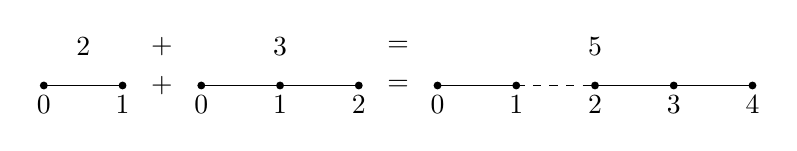
\begin{tikzpicture}
      \draw (0.5,0.5) node {$2$};
      \draw (1.5,0.5) node {$+$};
      \draw (3,0.5) node {$3$};
      \draw (4.5,0.5) node {$=$};
      \draw (7,0.5) node {$5$};
      \draw (0,0) node [below] {$0$} -- (1,0) node [below] {$1$};
      \draw (1.5,0) node {$+$};
      \draw (2,0) node [below] {$0$} -- (3,0) node [below] {$1$} -- (4,0) node [below] {$2$};
      \draw (4.5,0) node {$=$};
      \draw (5,0) node [below] {$0$} -- (6,0) node [below] {$1$};
      \draw [dashed] (6,0) -- (7,0);
      \draw (7,0) node [below] {$2$} -- (8,0) node [below] {$3$} -- (9,0) node [below] {$4$};
      \foreach \x in {0,1,2,3,4,5,6,7,8,9} {
        \fill (\x,0) circle (0.05);
      }
    \end{tikzpicture}
  \end{center}
  \caption{Ordinal sum of $2$ and $3$.}
  \label{fig:tikz-example}
\end{figure}

\begin{figure}
  \begin{center}
    \begin{tikzcd}
          A \arrow[rd] \arrow[r, "\phi"] & B \\
                                        & C
    \end{tikzcd}
  \end{center}
  \caption{Example of tikzcd diagram.}
  \label{fig:tikzcd-example}
\end{figure}

\subsection{...embed videos (WIP but functional)}
The package \verb|latexmlleeds| provides the command \ltxinline|\ldsHTML| to generate \HTML{} directly in your \verb|.tex| files. Hence you can copy and paste the \HTML{} code that your platform gives you for embedding the video. You may need to edit the \HTML{} code because it needs to be valid \XML{} as well, see \autoref{sub:latexmlleeds-sty} (it's just a few touches).

I recommend creating a command, like the \ltxinline|\includestream| below, to simplify embedding videos while also adding a link (the link is needed in PDF and EPUB). I have added a bit of \CSS{} to \verb|latexmlleeds.css| to make videos work well on all screens. Check the example \autoref{exa:embed-stream} and resize your browser to see how the video resizes accordingly. I will improve the \CSS{} in the near future to accommodate different video resolutions -- for now it expects $1280 \times 720$.
\begin{lstlisting}[style=latexml]
  % preamble
  \newcommand{\includestream}[2]{
  \ldsHTML{<div class="lds\_video"><div>
      <iframe
        src="https://web.microsoftstream.com/embed/video/#1?autoplay=false\&amp;showinfo=true"
        allowfullscreen="" width="1280" height="720">
      </iframe>
    </div></div>}
    Watch \href{https://web.microsoftstream.com/video/#1}{#2}
  }
  % document
  \includestream{ba6b8866-df29-4dea-a47e-13decc5cd409}{Mock recording for Models and Sets}
\end{lstlisting}

\subsection{...improve tables}
Tables generally work fine, although Mart\'in managed to trigger some interesting bugs using nested tables. As a general rule, if you are nesting tables, check if \verb|multirow| and \verb|multicol| (both supported by \LaTeXML{}) can give the same result.

  For accessibility, it is good practice to add hints about table headers. The \verb|latexml| provides a few commands like \ltxinline|\lxBeginTableHead{}| to mark rows or particular cells as table headers. This will improve the look of the \HTML{} table as well as improve its accessibility. The best way to understand these commands is to read the comments inside \verb|latexml.sty|.

\begin{exa}
  This is a mock table exercising a few aspects of \LaTeX{} tables, including borders, as well as \verb|tabularx| support.
  Code:
  \begin{lstlisting}[style=latexml]
\begin{table}[h!]
  \begin{tabularx}{\textwidth}{c|X||c}
    \lxBeginTableHead{} Header 1 & Header 2 & Header 3 \\
    \hline \lxEndTableHead{}
    Content & Content & Content \\
    More content & content & content \\
    \hline
  \end{tabularx}
  \caption{A table}
\end{table}
  \end{lstlisting}
  Output:
  \begin{table}[h!]
    \begin{tabularx}{\textwidth}{c|X||c}
      \lxBeginTableHead{} Header 1 & Header 2 & Header 3 \\
      \hline \lxEndTableHead{}
      Content & Content & Content \\
      More content & content & content \\
      \hline
    \end{tabularx}
    \caption{A table}
  \end{table}
\end{exa}
\section{Recap: how to compile this example}
\begin{lstlisting}[language=bash,caption={Generate the PDF}]
# I use latexmk, but pdflatex or your preferred engine will work
latexmk -pdf LaTeXML-Leeds
\end{lstlisting}
\begin{lstlisting}[language=bash,caption={Generate the EPUB}]
latexmlc --splitat=chapter \
  --destination=latexmlleeds/LaTeXML-Leeds.epub \
  LaTeXML-Leeds.tex
\end{lstlisting}
\begin{lstlisting}[language=bash,caption={Generate the HTML}]
latexmlc --mathtex --svg \
  --destination=latexmlleeds/LaTeXML-Leeds.html \
  LaTeXML-Leeds.tex
\end{lstlisting}
\begin{lstlisting}[language=bash,caption={Generate the HTML in two steps}]
latexml --destination=LaTeXML-Leeds.xml LaTeXML-Leeds.tex
latexmlpost --mathtex --svg \
  --destination=latexmlleeds/LaTeXML-Leeds.html \
  LaTeXML-Leeds.xml
\end{lstlisting}
\begin{lstlisting}[language=bash,caption={Do all the above steps in one go}]
# This uses the Makefile included in latexmlleeds
make
\end{lstlisting}

Meaning of the options:
\begin{description}
  \item[\texttt{{-}{-}splitat=section}] Split the document into a separate \HTML{} page per section, linked to each other. The value can be chapter, section, subsection, subsubsection.
  \item[\texttt{{-}{-}mathtex}] Add an equivalent \TeX{} code in maths formulas as annotation (it may slightly different from with the original code). With MathJax, the code appears by right-clicking on the formula and choosing ``Show Math As > Annotation > TeX''.
  \item[\texttt{{-}{-}svg}] Instruct \LaTeXML{} to use SVG as prefer image format. I have not tested this in real life, it may depend on having ImageMagick installed, and results may vary.
\end{description}
Further options that seem important enough (more will be added if they turn out to be relevant).
\begin{description}
  \item[\texttt{{-}{-}navigationtoc=(context|none)}] The value used in this guide is the default (\verb|none|). The value \verb|context| should produce a traditional navigation bar with links to all the chapters, and additional links to sections in the current chapter. I have not tried it yet.
  \item[\texttt{{-}{-}css=style.css}] Import the \CSS{} \verb|style.css| in every page.
  \item[\texttt{{-}{-}stylesheet=...}] Use an alternative \XSLT{} stylesheet in place of the standard ones. You probably do not want to touch this option: the important settings are already customised in \verb|LaTeXML-html5.xsl| (see \autoref{sub:xslt} to see what the customisations do on top of \LaTeXML{}).
\end{description}
For the full list of options, visit the \href{https://dlmf.nist.gov/LaTeXML/docs.html}{\LaTeXML{} documentation} or run \verb|latexml --help|, \verb|latexmlpost --help|, \verb|latexmlc --help|.

\section{Documentation}

\subsection{The \texttt{latexml} package}
\begin{lstlisting}[style=latexml,caption={Import \texttt{latexml} in the preamble}]
  \usepackage[nocomments]{latexml}
\end{lstlisting}

The package \verb|latexml| takes some options that will be passed to the \LaTeXML{} engine, such as \ltxinline|nocomment| (that strips the \ltxinline|%| comments away) or \ltxinline|mathparsespeculate|. Moreover, it offers a variety of commands. The most important one:
\begin{lstlisting}[style=latexml]
  \iflatexml
    % code only executed by latexml
  \else
    % code only executed by other engines
  \fi
\end{lstlisting}

\begin{exa}
  Code:
  \begin{lstlisting}[style=latexml]
    \usepackage{latexml}
    ...
    \begin{document}
    ...
    \iflatexml Great, you used \LaTeXML{} successfully!
    \else This is a boring PDF.\fi
  \end{lstlisting}
  Output:
  \begin{quote}
    \iflatexml Great, you used \LaTeXML{} successfully!
    \else This is a boring PDF.\fi
  \end{quote}
\end{exa}

For reference, \verb|latexml| also defines the following, although you can work very well without them. Just open \verb|latexml.sty| (it is very short) to see all the commands, a bit of documentation in the comments, and the occasional example. The \href{https://github.com/brucemiller/LaTeXML/tree/master/doc/manual}{source} of the \LaTeXML{} documentation is also a source of examples.
\begin{itemize}
  \item \ltxinline|\lxAddClass{class}| and \ltxinline|\lxWithClass{class}{content}| to add \CSS{} classes to the output;
  \item \ltxinline|\lxBeginTableHead|, \ltxinline|\lxEndTableHead| and variations to mark table headers and footers (read the \verb|latexml.sty| source for how to use them);
  \item \ltxinline|\lxFcn{code}|, \ltxinline|\lxID{code}|, \ltxinline|\lxPunct{code}| to help \LaTeXML{} understand the meaning of mathematical symbols (\LaTeXML{} recognises the meaning on its own, but every once in a while, there will be a symbol that is just too ambiguous: is $f(a+b)$ the function $f$ applied to $a+b$, or the number $f$ multiplied by $a+b$? keep an eye on the warnings during compilation);
  \item \ltxinline|\lxContextTOC|, \ltxinline|\lxNavbar{arg}|, \ltxinline|\lxHeader{arg}|, \ltxinline|\lxFooter{arg}| to customise the HTML pages (I have yet to figure out how they work);
  \item and a few other commands.
\end{itemize}

\subsection{The \texttt{latexmlleeds} package}
\label{sub:latexmlleeds-sty}
\begin{lstlisting}[style=latexml,caption={Import \texttt{latexmlleeds} in the preamble}]
  \usepackage{latexmlleeds}
\end{lstlisting}

\verb|latexmlleeds| makes \LaTeXML{} include \verb|latexmlleeds.css| (see \autoref{sub:css}) and it offers some additional functionality.

\subsubsection{Outputting \HTML{} code}
\ltxinline|\ldsHTML{html}| outputs \ltxinline|html| argument directly as \HTML{} code. The \ltxinline|html| is only processed by \LaTeXML{} and ignored by other engines. The \LaTeXML{} processing is done by \verb|latexmlleeds.sty.lxtml|, which is a short Perl file you do not need to touch.
\begin{exa}
  Code:
  \begin{lstlisting}[style=latexml]
    This sentence appears in all versions.
    \ldsHTML{<span>But this part is
      <strong>only in the HTML outputs</strong>.</span>}
  \end{lstlisting}
  Output:
  \begin{quote}
    This sentence appears in all versions.
    \ldsHTML{<span>But this part is
    <strong>only in the HTML outputs</strong>.</span>}
  \end{quote}
\end{exa}

Some notes:
\begin{itemize}
  \item The \HTML{} must be written in ``\XML{} serialisation'', hence all tags must be closed (e.g.\ \verb|<br>| must be written as \verb|<br/>|) and all attributes must have a value (e.g.\ \verb|allowfullscreen| must be written \verb|allowfullscreen=""|).
  \item The content must be written inside \HTML{} elements. Any text not contained in an element will be dropped. If in doubt, put \verb|<span>...</span>| around your \HTML{}.
  \item The \HTML{} is still interpreted as \LaTeX{} code, hence it must be escaped appropriately. For instance, every \ltxinline|{| must be replaced by \ltxinline|\{|; every \ltxinline|&| must be replaced by \ltxinline|\&| (and probably be written as \ltxinline|\&amp;| -- you must write correct \HTML{}!).
\end{itemize}

\begin{exa}[Embed Stream videos]\label{exa:embed-stream}
  This is only a proof of concept, but already functional: it embeds a video directly into \HTML{} and EPUB, and provides a link in all contexts (note that embedded videos may not work everywhere, especially with EPUB, so always include the link). The code is accompanied by some extra \verb|<div>|'s and some \CSS{} inside \verb|latexmlleeds.css| to make the video responsive (the additional code is taken from Microsoft Stream). You should the code to match the resolution of your videos (mine is $1280 \times 720$).
  \begin{lstlisting}[style=latexml]
    % preamble
    \newcommand{\includestream}[2]{
    \ldsHTML{<div class="lds\_video"><div>
        <iframe
          src="https://web.microsoftstream.com/embed/video/#1?autoplay=false\&amp;showinfo=true"
          allowfullscreen="" width="1280" height="720">
        </iframe>
      </div></div>}
      Watch \href{https://web.microsoftstream.com/video/#1}{#2}
    }
    % document
    \includestream{ba6b8866-df29-4dea-a47e-13decc5cd409}
    {Mock recording for Models and Sets}
  \end{lstlisting}

  Output:
  \begin{quote}
    \newcommand{\includestream}[2]{
      \ldsHTML{<div class="lds\_video"><div>
          <iframe 
            src="https://web.microsoftstream.com/embed/video/#1?autoplay=false\&amp;showinfo=true"
            allowfullscreen="" width="1280" height="720">
          </iframe>
        </div></div>}
      Watch \href{https://web.microsoftstream.com/video/#1}{#2}
    }
    \includestream{ba6b8866-df29-4dea-a47e-13decc5cd409}
    {Mock recording for Models and Sets}
  \end{quote}
\end{exa}

\subsubsection{Workaround for TikZ pictures}
\label{ssub:TikZ}
If your TikZ figures are crashing \LaTeXML{}, importing \verb|latexmlleeds| with the following options will hide your TikZ figures from \LaTeXML{}, while it will make \verb|pdflatex| output the images in the \verb|images| subfolder in PDF and SVG format. You will need to manually hide \ltxinline|\usepackage{tikz}| from \LaTeXML{} using \ltxinline|\iflatexml| and ensure that you call \ltxinline|\usetikzlibrary{external}|. See \autoref{sub:tikz-howto}, or the source of this file, for an example.
\begin{description}
  \item[\texttt{tikzextern}] When compiling to PDF, make TikZ export all TikZ pictures as images named \verb|images/TikZ-#.pdf| (where \verb|#| is a number); when compiling with \LaTeXML{}, replace all TikZ pictures with the corresponding images in \verb|images/TikZ-#.pdf|. \textbf{You need to pass the option \texttt{-shell-escape} to \texttt{pdflatex} for this to work.}
  \item[\texttt{tikzextern=prefix}] Same as above, but replaces \verb|images/TikZ-| with \verb|prefix|.
  \item[\texttt{tikz2svg}] When compiling to PDF, also create an SVG version of the images by running command \verb|pdf2svg images/TikZ-#.pdf images/TikZ-#.svg| (or \verb|pdf2svg prefix#.pdf images/prefix#.svg|). \textbf{You need to install \texttt{pdf2svg} for this to work.}
  \item[\texttt{tikz2svg=command}] Same as above, but run \verb|command| instead of \verb|pdf2svg|.
  \item[\texttt{tikzscale=factor}] When converting to SVG, scale the output for the web by \verb|factor|. The default setting if you do not pass \verb|tikzscale| is \verb|1.333| (since PDF content uses 72 points per inch, while web content uses 96 points per inch).
  \item[\texttt{tikzcd}] Enable an additional workaround for the \verb|tikz-cd| library, which is not compatible with \verb|tikzextern| out of the box.
\end{description}
Note that you must create the \verb|images| folder (or whatever folder appears in your \verb|prefix|) before running \verb|pdflatex|.

\subsection{The \texttt{LaTeXML-html5.xsl} customisations}
\label{sub:xslt}
Normally, you do not need to care about this file. The \verb|LaTeXML-html5.xsl| \XSLT{} stylesheet does three things:
\begin{itemize}
  \item include the latest version of MathJax 3 as well as a compatibility polyfill for IE11;
  \item make \HTML{} lists more accessible by ignoring custom enumerations (i.e., the \ltxinline|(a)| in \ltxinline|\item[(a)]|; you should modify your \CSS{} to do custom enumerations in \HTML{});
  \item add modern HTML5 tags to make the output more mobile friendly while replacing the outdated \verb|Content-type| meta tag with \verb|charset|.
\end{itemize}
The \XSLT{} may be updated in the future to improve a few aspects of the resulting \HTML{}; for instance, we might discover that offloading the maths parsing entirely to MathJax is better overall, and this can only be done by tweaking the \XSLT{}.

\subsection{The \texttt{latexmlleeds.css} customisations}
\label{sub:css}
This is where you can tweak the appearance of your \HTML{} files. For now, the basic \verb|latexmlleeds.css|
\begin{itemize}
  \item sets the font to sans serif (trying to pick the best font available);
  \item reduces the margins to a minimum;
  \item sets the maximum text width to about 80 characters;
  \item reduces the margins on the lists;
  \item removes indentation;
  \item implements responsive styling for embedded videos (see \autoref{exa:embed-stream}).
\end{itemize}
This styling has only been tested with the \verb|article| class and on Edge and Chrome, so further tweaks may be needed.

\section{Good practices}
\begin{itemize}
  \item Follow Martin's recommendations about fonts, tables, margins, and so on.
  \item Use semantic \LaTeX{} commands as much as possible (\ltxinline|\chapter|, \ltxinline|\section|, \ltxinline|\newtheorem|).
  \item Although not strictly needed, it is better to restrict yourself to MathJax supported commands in math mode. In this way the students will be able to copy and paste your \TeX{} code from the lecture notes to the discussion boards, once they learn how to do so. See the MathJax documentation for the full list.
\end{itemize}

\section{Other documentation}
\begin{itemize}
  \item \href{https://dlmf.nist.gov/LaTeXML/docs.html}{\LaTeXML{} documentation}
  \item List of packages \href{https://dlmf.nist.gov/LaTeXML/manual/included.bindings/}{supported by \LaTeXML{}} (note that some implementations are not complete)
  \item \href{http://docs.mathjax.org/en/v2.7-latest/}{MathJax v2.7} documentation
  \item List of \LaTeX{} commands \href{http://docs.mathjax.org/en/v2.7-latest/tex.html#supported-latex-commands}{supported by MathJax v2.7}
  \item \href{http://docs.mathjax.org/en/v3.1-latest/}{MathJax v3.1} documentation
  \item List of \LaTeX{} commands \href{http://docs.mathjax.org/en/v3.1-latest/input/tex/macros/index.html}{supported by MathJax v3.1}
\end{itemize}

\end{document}
